\paragraph{Thực nghiệm với Google Stock Price} \hfill \\
Dự báo giá cổ phiếu là một trong những bài toán khó nhất do tính nhiễu và sự biến động mạnh của thị trường tài chính.

\paragraph{Mô hình Conv1D + LSTM} \hfill \\
Chúng ta kết hợp lớp \textbf{Conv1D} để lọc nhiễu và trích xuất các đặc trưng cục bộ (pattern) ngắn hạn, sau đó đưa vào lớp \textbf{LSTM} để học các xu hướng dài hạn. Cửa sổ quan sát được thiết lập là 60 ngày (\textbf{LOOK\_BACK = 60}).

\paragraph{Kết quả và Phân tích} \hfill \\
Mô hình đạt \textbf{R² score là 0.9745} và \textbf{Test RMSE là 22.37 USD}. Biểu đồ dự báo cho thấy mô hình bắt kịp các xu hướng tăng giảm chính của mã cổ phiếu GOOGL.

\begin{figure}[H]
    \centering
    \begin{minipage}{0.48\textwidth}
        \centering
        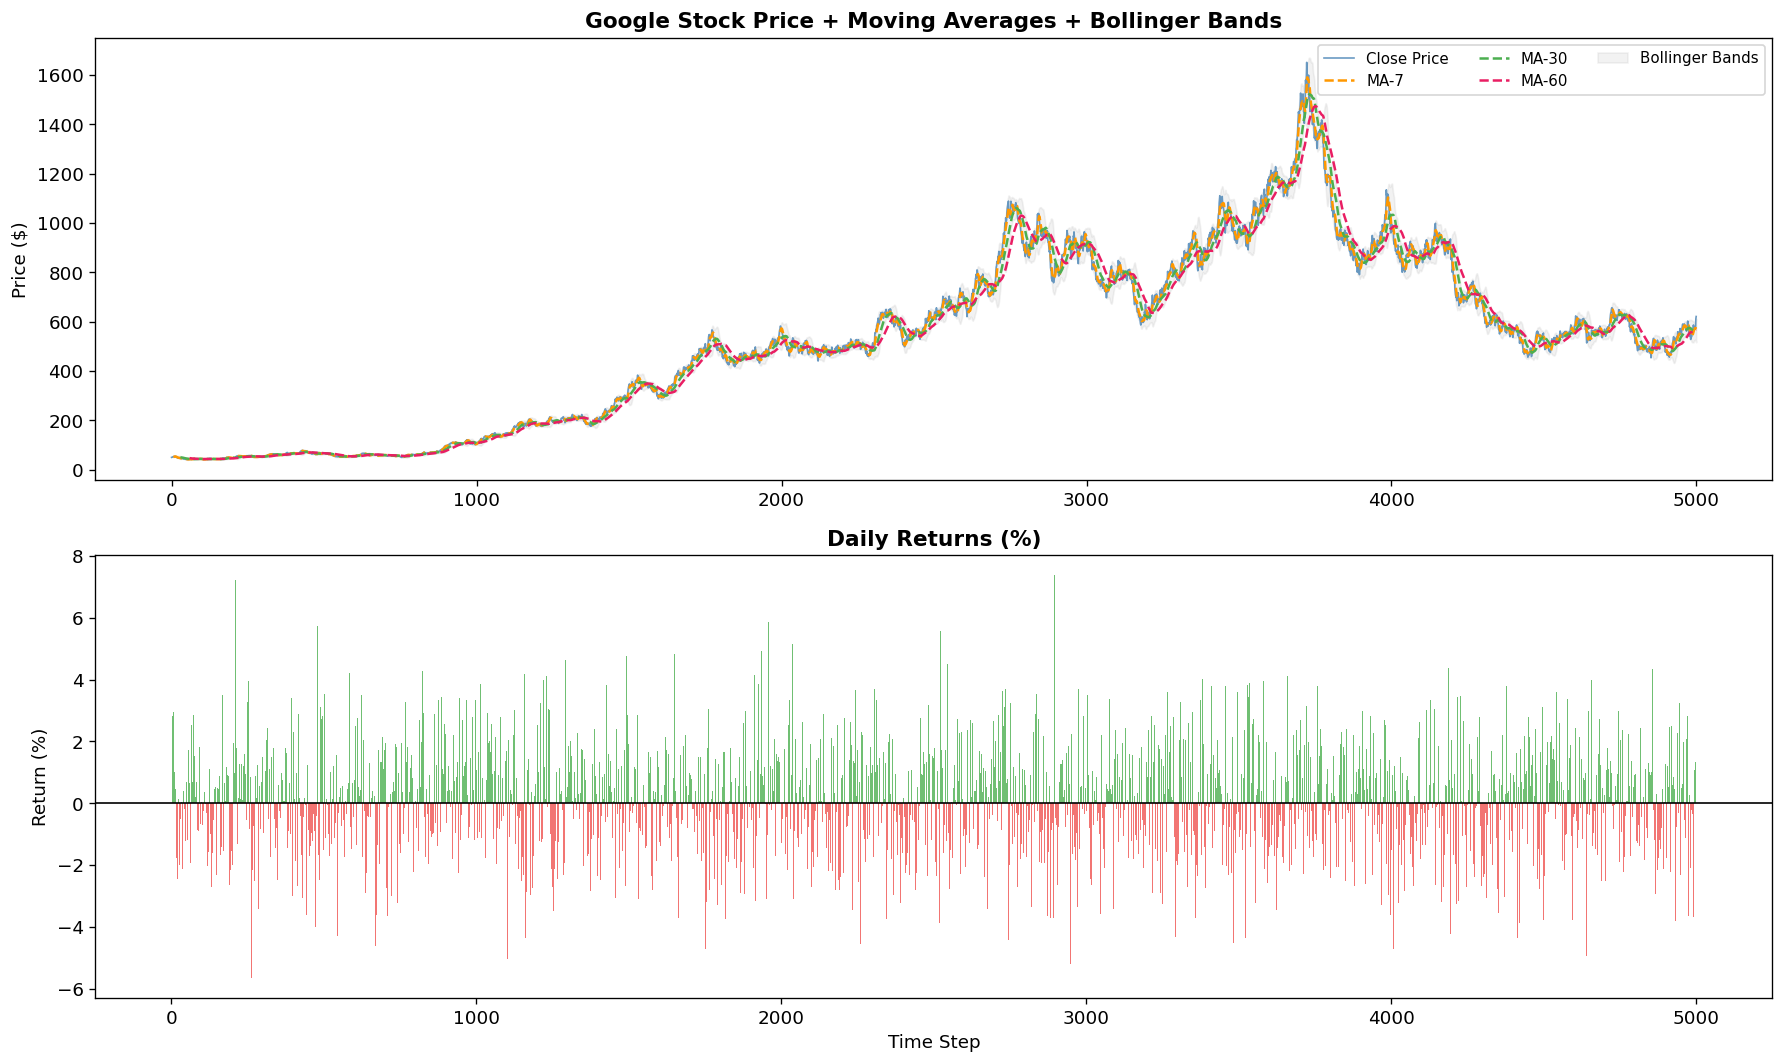
\includegraphics[width=\linewidth]{Chương_4/results/google_stock/01_stock_eda.png}
        \caption{Biến động giá cổ phiếu Google (Lịch sử)}
        \label{fig:stock_eda}
    \end{minipage}
    \hfill
    \begin{minipage}{0.48\textwidth}
        \centering
        \includegraphics[width=\linewidth]{Chương_4/results/google_stock/02_returns_volatility.png}
        \caption{Phân tích lợi nhuận và độ biến động}
        \label{fig:stock_vol}
    \end{minipage}
\end{figure}

\begin{figure}[H]
    \centering
    \includegraphics[width=0.8\linewidth]{Chương_4/results/google_stock/03_forecast_results.png}
    \caption{Kết quả dự báo giá cổ phiếu trên tập kiểm tra}
    \label{fig:stock_forecast}
\end{figure}


\paragraph{Phụ lục: Quy trình thực nghiệm chi tiết} \hfill \\
Dưới đây là các bước triển khai chi tiết trên môi trường Jupyter Notebook:

\begin{figure}[H]
    \centering
    
\includegraphics[width=0.9\linewidth]{Chương_4/docs/ch4/15.png}
    \caption{Tải dữ liệu tài chính: Đọc lịch sử giá cổ phiếu Google (GOOG) bao gồm các cột giá Open, High, Low, Close và Volume.}
\end{figure}

\begin{figure}[H]
    \centering
    
\includegraphics[width=0.9\linewidth]{Chương_4/docs/ch4/16.png}
    \caption{EDA giá cổ phiếu: Trực quan hóa sự tăng trưởng dài hạn và các giai đoạn biến động mạnh của thị trường.}
\end{figure}

\begin{figure}[H]
    \centering
    
\includegraphics[width=0.9\linewidth]{Chương_4/docs/ch4/17.png}
    \caption{Feature Engineering nâng cao: Tính toán các chỉ số bổ sung từ giá đóng cửa và khối lượng giao dịch.}
\end{figure}

\begin{figure}[H]
    \centering
    
\includegraphics[width=0.9\linewidth]{Chương_4/docs/ch4/18.png}
    \caption{Tiền xử lý chuỗi: Chuẩn hóa và tạo cửa sổ dữ liệu quan sát (`LOOK\_BACK = 60`) để dự báo xu hướng tiếp theo.}
\end{figure}

\begin{figure}[H]
    \centering
    
\includegraphics[width=0.9\linewidth]{Chương_4/docs/ch4/19.png}
    \caption{Kiến trúc Conv1D-LSTM: Kết hợp lớp Convolution 1D để lọc nhiễu và LSTM để ghi nhớ các đặc trưng dài hạn.}
\end{figure}

\begin{figure}[H]
    \centering
    
\includegraphics[width=0.9\linewidth]{Chương_4/docs/ch4/20.png}
    \caption{Quá trình huấn luyện: Nhật ký thực thi cho thấy sự sụt giảm nhanh chóng của MSE Loss trên cả hai tập dữ liệu.}
\end{figure}

\begin{figure}[H]
    \centering
    
\includegraphics[width=0.9\linewidth]{Chương_4/docs/ch4/22.png}
    \caption{Kết quả Training History: Đồ thị Loss hội tụ tốt sau 20 epochs, không xuất hiện hiện tượng Overfitting.}
\end{figure}

\begin{figure}[H]
    \centering
    
\includegraphics[width=0.9\linewidth]{Chương_4/docs/ch4/23.png}
    \caption{Tổng kết thực nghiệm: Bản tóm tắt trực quan bao gồm Lịch sử huấn luyện, Dự báo toàn cục và Biểu đồ tương quan Scatter Plot ($R^2 = 0.9745$).}
\end{figure}
